%!TEX root = ../thesis.tex
%*******************************************************************************
%*********************************** First Chapter *****************************
%*******************************************************************************

\chapter{Introduction \label{chap:1}}  %Title of the First Chapter

\ifpdf
    \graphicspath{{Chapter1/Figs/Raster/}{Chapter1/Figs/PDF/}{Chapter1/Figs/}{Chapter1/Figs/Vector/}}
\else
    \graphicspath{{Chapter1/Figs/Vector/}{Chapter1/Figs/}}
\fi



A new field of research in material science and condensed matter physics was formed after the synthesis of graphene in 2004 \cite{Novoselov666,Novoselov26072005}. This field is named Two-dimensional (2D) material due to the fact that graphene is a single atomic-layer crystal. The synthesis itself together with the phenomenal properties of graphene has leaded to a Nobel Price in physics rewarded to A. K. Geim and K. S. Novoselov \cite{Geim2007}. Since then, the field is expanding with the involvement of researcher not only from young community, but also from experts who have been working on materials like graphite, fullerenes and carbon nanotubes which are strongly graphene related. In the last several years, researches focused on graphene and related topics increasing rapidly, see \autoref{fig:grpapers}. While a part of these effects have been making to explore more on the graphene itself and its applications, some other parts were put on discovering new 2D materials. It has been evidenced from graphene, same material having different dimensionality can have different properties. Therefore, many materials with hidden properties which will only manifest itself at other dimensions yet to be discovered. 


\begin{figure}[htbp!] 
\centering  
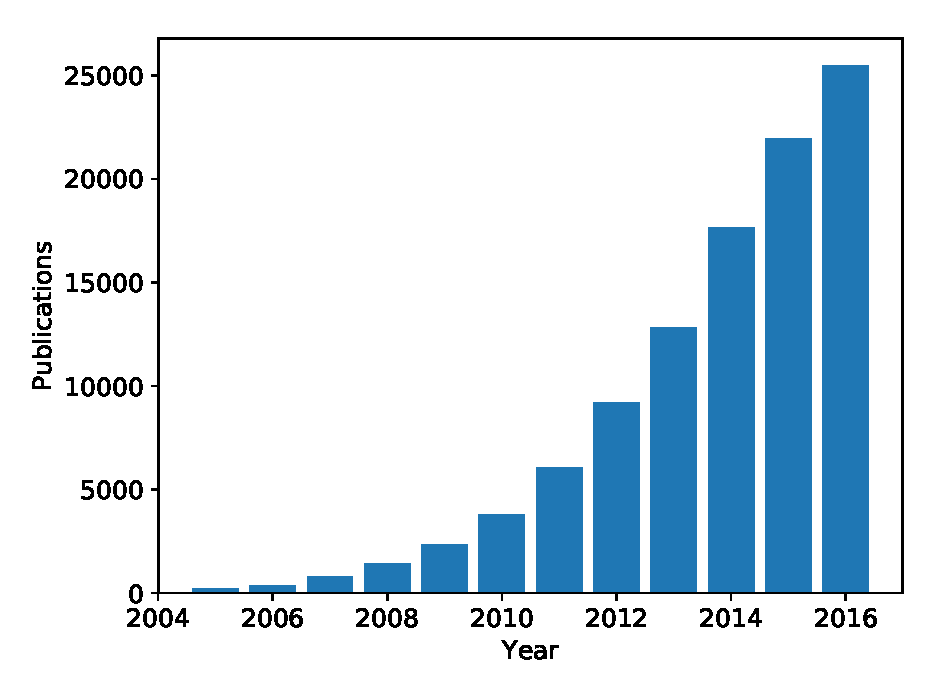
\includegraphics[width=0.7\textwidth]{graphene_papers.eps}
\caption[Graphene publications]{Graphene related publications during the last decade. Source ISI Web of Science. \protect\footnotemark }  
\label{fig:grpapers}
\end{figure} 

On the other hand, with the advent of powerful supercomputer facilities, calculations that seems impossible to finish in a reasonable time now has been made accessible. At the same time, given the accuracy of the calculations is the most crucial aspect of computational physics, especially when the results are related to the prediction the real properties of materials, researchers and programmers have been making important progress to make sure theories and its implementation are correct and the results they yield are within acceptable precision. Equipped with these tools, theoretical predictions on the structure and the properties of material have served well on discovering unexplored features. Moreover, detailed characterizations at atomic scale benefits the experimental results to make it more convincing, or even sometimes to explain the unexpected results.

\footnotetext{This result is obtained by searching for "graphene" in the topic field of Web of Science.}

Considering all mentioned, it is a sound approach to apply the state-of-the-art computational methods that accompanied with high-performance supercomputer facilities to investigate the physical properties of novel 2D materials. This thesis is a summary of several works which has accomplished during my PhD study and were initiated to this end. The thesis is organized as followed: For the rest of this chapter, I will first introduce graphene and some post-graphene materials that discovered right after graphene and, briefly, methods used to synthesis 2D materials. The following \autoref{chap:2} will present the computational methods, the theory behind and the implementations of them. In \autoref{chap:3}, I will discuss several general properties of 2D materials. The next two chapters will be the main results from my works. Starting from specific properties targeting at specific novel 2D materails in \autoref{chap:4}, and followed by modification of physical properties of 2D materials in \autoref{chap:5}. Conclusions for the thesis will be given in the last chapter.

\section{Graphene}

Graphene is composed of carbon (C) atoms arranged on a hexagonal lattice. Each C atoms bond to three neighbouring C atoms. Graphene is one single atomic layer of graphite, see \autoref{fig:gra_grap}. These layers in graphite are stacked on top of another through weak physical bonding, whereas within each layer C atoms are hold together by strong chemical bonding. As a result, it is possible to just isolate single layer from graphite without damaging the layer itself. 

\begin{figure}[htbp!] 
\centering  
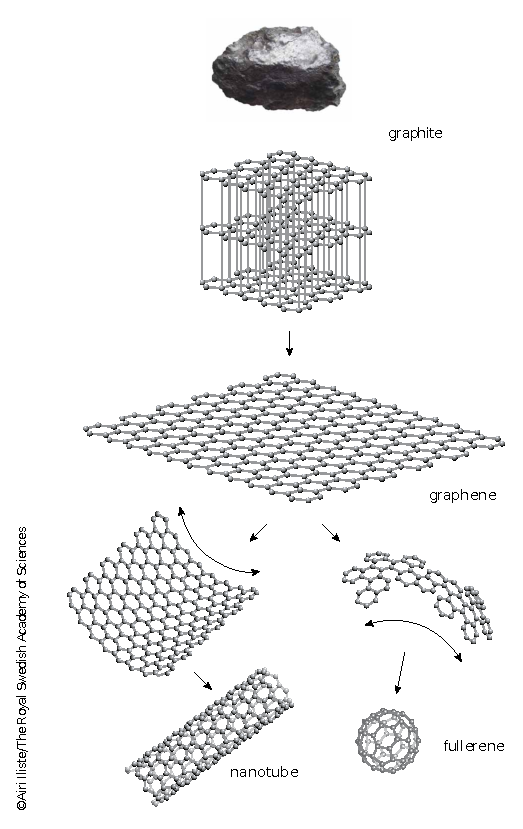
\includegraphics[width=0.7\textwidth]{gra_grap.eps}
\caption{Relation of graphite, graphene, fullerene and nanotube. Source the Nobel prize in physics 2010 \cite{gra_grap}. }  
\label{fig:gra_grap}
\end{figure} 


\subsection{History}

The story of graphene can be trace back to the discover of graphite around 1564 in England\cite{petroski1990pencil}. Ever since, people have been using the graphite, the tip of a pencil, for writing and drawing. The black trace left behind by pencil they are actually stacks of graphite and graphene, by chance even a single layer graphene can present.  Apart from being a part of a pencil, graphite certainly has been holding a important position in technology and industry due to its rich chemistry, low friction, high electrical and thermal conductivity etc.. On the other hand, the synthesis of single layer graphene seems to be discouraged by both experimental and theoretical limitation. On the experiments, there are have been attempts\cite{Krishnan1997,Ohashi1997,Dresselhaus2002,Shioyama2001} to isolate graphene or ever grow it. However, they were mostly failed on control of the number of layers and identifying graphene itself.  Addition to these experimental difficulties, on the theory, it was believed that strictly 2D material should not exist due to a divergence in the thermal fluctuation in 2D materials that will make them not stable \cite{Peierls1935,Landau1937,Mermin1968}. Nevertheless, graphene was still considered as theoretical model. for example, \citet{Wallace1947} was the first one to study the band structure of graphene \cite{CastroNeto2009} and found some of the interesting properties like semimetallic band structure. 

Although not in the form of graphene, the single atomic layer of graphite has been already seen and studied in other forms although includes certain type of characteristic defect that differ it from graphite, e.g. fullerene and nanotube, see \autoref{fig:gra_grap}. Flulerene is a C modelue has a quasispherical hollow ball shape. It is composed of both six- and five-folded C rings, where the latter give positive curvature and made closed surface possible which resemble a football\cite{Kroto1985,Lamb1990}. The Nobel prize in chemstry of year 1996 was award to Harold W. Kroto, Robert F. Curl and Richard E. Smalley for their discovery of fullerene. The method to produce a large quantity of fullerene, i.e. arc-discharge method\cite{Lamb1990}, also results in another important carbon allotrope: carbon nanotubes\cite{Iijima1993}. Despite sharing similar production method with fullerene, carbon nanotubes are more close to graphene in a sense that it can be construct by rolling up finite graphene sheet into a hollow tube as its name suggested, and more importantly, these two both free of pentagonal C rings while fullerene must have a certain number. Carbon nanotubes are observed to have micrometer in lengths and nanometer in diameters and having either metallic or semiconducting nature depending on its edges. Individual nanotube has a Young's modulus of 0.64 TPa and it is 56 times stronger than steel wire\cite{Baughman787}.

In 2004, the situation has changed completely for graphene with the successfully isolated single layer graphene from graphite by A. K. Geim and K. S. Novoselov at Manchester University using a simple micromechanical cleavage method. The key ingredient, except for sophisticated experimental control, as compared to the previous failures\cite{Krishnan1997,Ohashi1997} in this case is that the Si wafer under the graphene made it easier to identify graphene\cite{Geim2007}. The synthesis of graphene itself already is a ground-breaking achievement, however, what excited the researcher the most is the extraordinary properties of graphene. In the following section, I will summarized some of them to illustrate this point.

\subsection{Physical properties}

As mentioned previously, graphene is the single atomic layer of graphite. It is made of three-folded C atoms that are arranged in a honeycomb lattice\footnote{honeycomb lattice is not a bravais lattice.}, or a hexagonal bravais lattice with two atoms per site, see \autoref{fig:gra_lat}. graphene has uniform bond lengths and bond angles which are 1.42 \AA~and 120\textdegree, respectively. Every atom has same local environment, however, adjacent atoms are not equivalent. $a\Gamma\Sigma\delta$

\begin{figure}[htbp!] 
\centering  
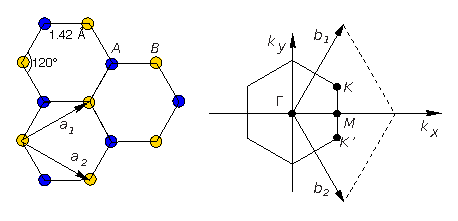
\includegraphics[width=0.7\textwidth]{gra_lat.eps}
\caption{Graphene lattice and its Brillion zone. Source \cite{CastroNeto2009}. }  
\label{fig:gra_lat}
\end{figure} 

\subsection{Physical properties}
\section{Post-graphene Materials}
\subsection{Functionized Graphene}
\subsubsection{Graphane}
\subsubsection{Fluorographene}
\subsection{Boron Nitride}
\subsection{Silicene and Germanene}
\subsection{Transition Metal Dichalcogenides}
\section{0D and 1D from 2D: buckyballs, nanotubes and nanoribbons}
\section{Synthesis methods}
